\section{User Interface}
\label{sec:designUI}
Even though we had an agreement, that the ITC group was to create an Android application implementing our programme, our project still had to be able stand on its own. We therefore decided to create a user interface displaying the programme's capabilities. 

The user interface (UI) for Stegosaurus is created in Visual Studio using C\# and WinForms.
In one of our previous experiments, we had created a very basic UI.
The only functionality of that UI was to show the cover image, the image to be hidden in the cover and the final output.

Something the experiment lacked was a choice of encoding.
For example, whether they would like to use the least significant bit method or our graph theoretical method.
Therefore, the final design should include several different options, so as to customise the encoding of their image to what suits their requirements.

Another thing lacking in previous designs has been a guide or explanation throughout the programme and description of its joint functionality.
Previous versions have been less complex and perhaps did not require much explanation.
However, now as the programme will have a larger set of settings, we believe that it should be a requirement to have a short explanation of these, what impact they will have on the end result and what the programme will do in general.

All of these things should illustrate to the user how the programme works and what it is doing while running.

\subsection{Design}

The form as shown in figure \ref{fig:LSBForm} is what our UI looked like for our LSB experiment.
We are taking the main ideas from this, where we show the user the images or files they have selected and the final product. This should ensure them, that the correct files have been selected and the encoding process has succeeded.
\begin{figure}
	\centering
	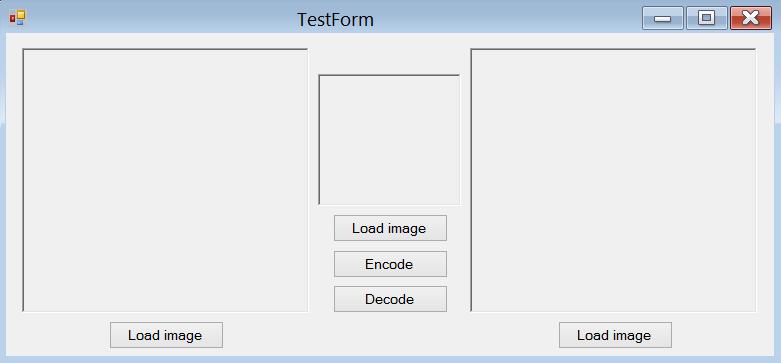
\includegraphics[width=\textwidth]{figures/LSBForm.png}
	\caption{This is the form for our LSB experiment, which acted as inspiration to our final design.}
	\label{fig:LSBForm}
\end{figure}
We decided, however, that it was confusing to have three separate load buttons.
As shown in figure \ref{fig:LSBForm} above, the cover image is uploaded in the left side, the message in the middle and the encoded image on the right.
When you wanted to decode the image, the encoded image had to be uploaded using the load-button to the right. This led to a confusing user experience.
Because of this we have decided to only have two buttons, one for loading an image that is to be either encoded or decoded and another for only getting the hidden message.

We have furthermore decided to include extra features to our overall design making use of the functionality of our programme's encoder and decoder.
These features include giving the user options to use their own Huffman and quantization tables to control the encoding process with precision.

To do this, we decided that creating an options form would be ideal when it comes to guiding the user through this extended functionality.
The options form would consist of a choice of encoding method, a quality-setting for use when encoding using our graph-theoretic method, customisation of Huffman and quantization tables.
However, there is also an option to reset all settings to default, if the user in question has no specific preferences or made an error.

After their message has been encoded, there is, naturally, a need to be able to decode it after the encoding process.
This means that the programme should be able to present these options to the user as openly as possible, as these are the key features of the programme.

As something more general, we have created a basic help guide to explain to the user how the programme works, and a short description of what each feature entails.
Within this menu item, there will also be an \textit{About} window that gives a short description of the programme, who it is by and under which circumstances it has been made.

Something that is absolutely fundamental to the programme, is showing the user the images they provide and the image they produce.
This visual representation gives the user reassurance that they have chosen the correct files.

Likewise, another feature, that we deem to be a rather important visual representation is the quality of encoding.
Therefore, we have decided to have a slider to show what level of quality the programme will encode with.

Saving of all these custom settings of course needed to be a function of the programme as they can be quite time-consuming to set and this is now done as soon as the programme is closed.

The following list is what the user interface will include:

\begin{description}
\item[Main form]
We wanted to make the main form as simple as possible. Therefore we have a single button for loading images. Additionally, there is also a single button for both encoding and decoding, this option can be selected by using the radio buttons. Also there is an option for encoding text, or simply encode a file.

\item[LSB or Graph Theory Method]
The user will be able to switch between the two different methods in the options form. This is an improvement over our initial design that utilised two separate tabs on the main form, one for encoding or decoding using the LSB method and one for the GT method. This resulted in a simpler interface with almost identical functionality being less split across the programme. This improvement is made possible by the OOP design of the encoders and decoders, having the various ways of encoding/decoding available from the same interface.

\begin{figure}
	\centering
	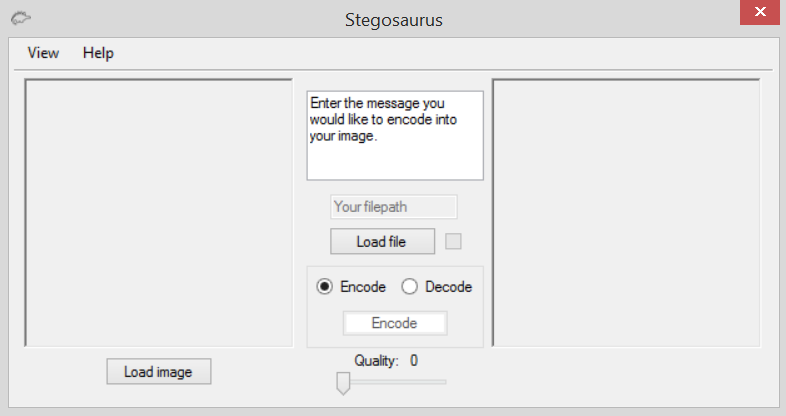
\includegraphics[width=1\textwidth]{figures/StegoMainForm.png}
	\caption{This is how the user will meet our graph theoretical method and LSB, where the message to be encoded no longer has to be an image, but can be a text message written directly in the programme or any sort of file freely selected}
	\label{fig:StegoMainForm}
\end{figure}

\item[Quality setting]
A slider shows the user what quality setting currently used when encoding JPEG images. 
This slider was initially planned to only be a part of the main form, but has since been moved to options as well as the main form for the graph theoretical method, as we decided it was as much a custom option as the Huffman and quantization tables.

\item[Quantization Tables]
A difficulty that arose when deciding on these features was how we were going to make it possible for a user to input their custom quantization and Huffman codes.

An initial idea included a CSV-file (Comma Separated Values file), but we decided that for quantization tables, it was ideal and no trouble to have the user customise their tables by typing them in text boxes, as the size of each quantization table is always 64 for both the luminance and chromium channels. This can be seen in figure \ref{fig:StegoOptionQuant}.


\begin{figure}[H]
	\centering
	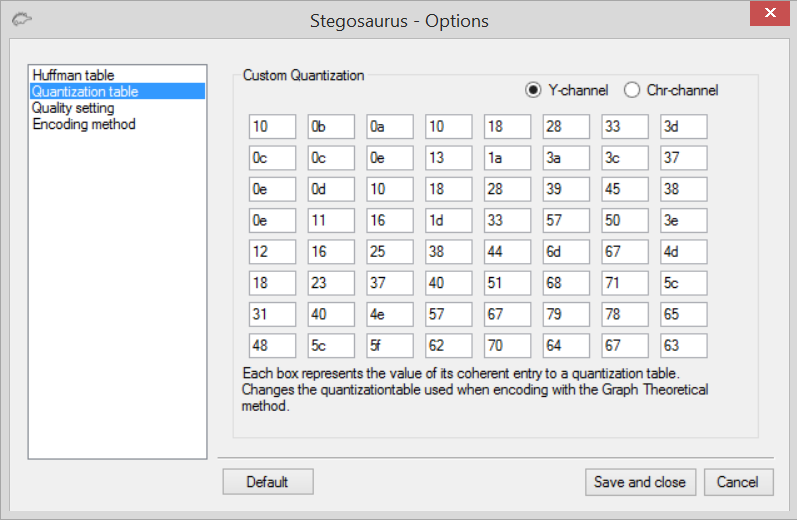
\includegraphics[width=1\textwidth]{figures/StegoOptionQuant.png}
	\caption{This is how the custom quantization table is shown to the user in the options setting form.}
	\label{fig:StegoOptionQuant}
\end{figure}

\item[Huffman Tables]

Huffman tables requires a similar design to quantization tables. There are four radio buttons to switch between the four different channels. Text boxes have been set up to be able to take in a string from the user. However, as the sizes of the Huffman tables vary, it is necessary to have a button that allows the user to add rows as needed. Huffman table customisation can be seen in figure \ref{fig:StegoOptionHuff2}.

\begin{figure}[H]
	\centering
	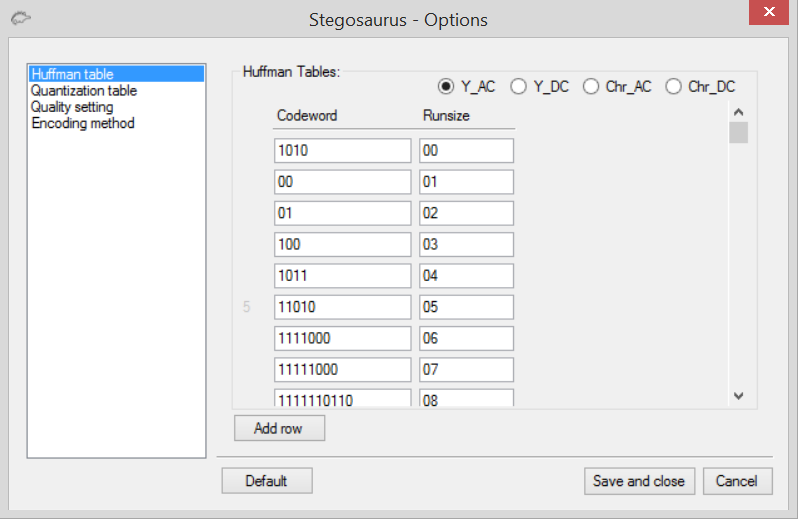
\includegraphics[width=1\textwidth]{figures/StegoOptionHuff2.png}
	\caption{The picture above shows how the user will see the Huffman table options setting.}
	\label{fig:StegoOptionHuff2}
\end{figure}

\item[Help form]
A very general description of what the programme does and descriptions of the different settings in the options form.
We believe this to be important to the overall understanding of how the programme is to be used; something that our previous experiments have not had.
\end{description}

There were some things with the UI that has been seen as problematic.
Although the programme did tell the user that an error occurred when they tried to save an illegal set of settings, it did not save any of the settings but reverted to the previous set. That meant that the user had to reconfigure everything from even just one single mistake.

This cumbersome way of handling this was caused by a poor, overall structure, where the main form was handling the actual saving of the settings, not the options-form.
This far from ideal structure meant that it was required to send variable values back and form between the two forms.
This has been improved on and the options-form now handles everything that has to do with settings, including saving.

This new interface has advantages over previous interfaces in our experiments throughout our process, but there are still some features that could be included, not to improve the programme, but the overall user experience.
